Bij cilindercoordinaten is een extra \textbf{factor $\bm r$} verplicht als je integreert, bij bolcoordinaten $\rho^2 \sin \phi$
Om bolco\"ordinaten te onthouden, gebruik poolco\"ordinaten en druk $r$ uit in $\rho$ en $\phi$ met behulp van onderstaand driehoekje, zodat $r=\rho \sin \phi$, en vul deze in, in poolco\"ordinaten $r \cos \theta,r \sin \theta$ om $x$ en $y$ te krijgen.
Vind de $z$-co\"ordinaat op dezelfde manier zodat $z=\rho \cos \phi$.
Zie figuur~\ref{bolMMa} in de appendix om je gekozen co\"ordinaten te controleren met Mathematica.
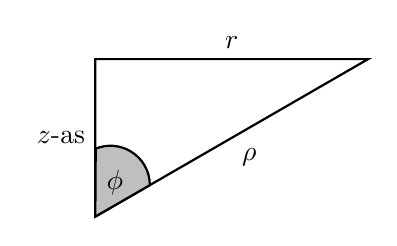
\begin{tikzpicture}[thick]
    \draw(0,0)
    -- (90:2cm) node[midway,left]{$z$-as}
    -- (30:4cm) node[midway,above]{$r$} % node of point
    -- (0,0) node[midway,below right]{$\rho$};
    \draw[fill=lightgray, thick] (0,0)
    -- (30:0.8cm) arc (0:112:0.5cm) node at (60:0.5cm) {$\phi$}
    -- cycle;
\end{tikzpicture}